% Schematic representation of Chip Layout
% Modified from a version created by Henrik Kröger, 
%https://github.com/derhedwig/fiberoptics/blob/master/auswertung.tex
% Author: Orlando Torres (2016)

\documentclass{standalone}
\usepackage{amsmath} % Required for \varPsi below
\usepackage{tikz,pgfplots}
\usetikzlibrary{calc}
\usetikzlibrary{patterns}

\begin{document}
  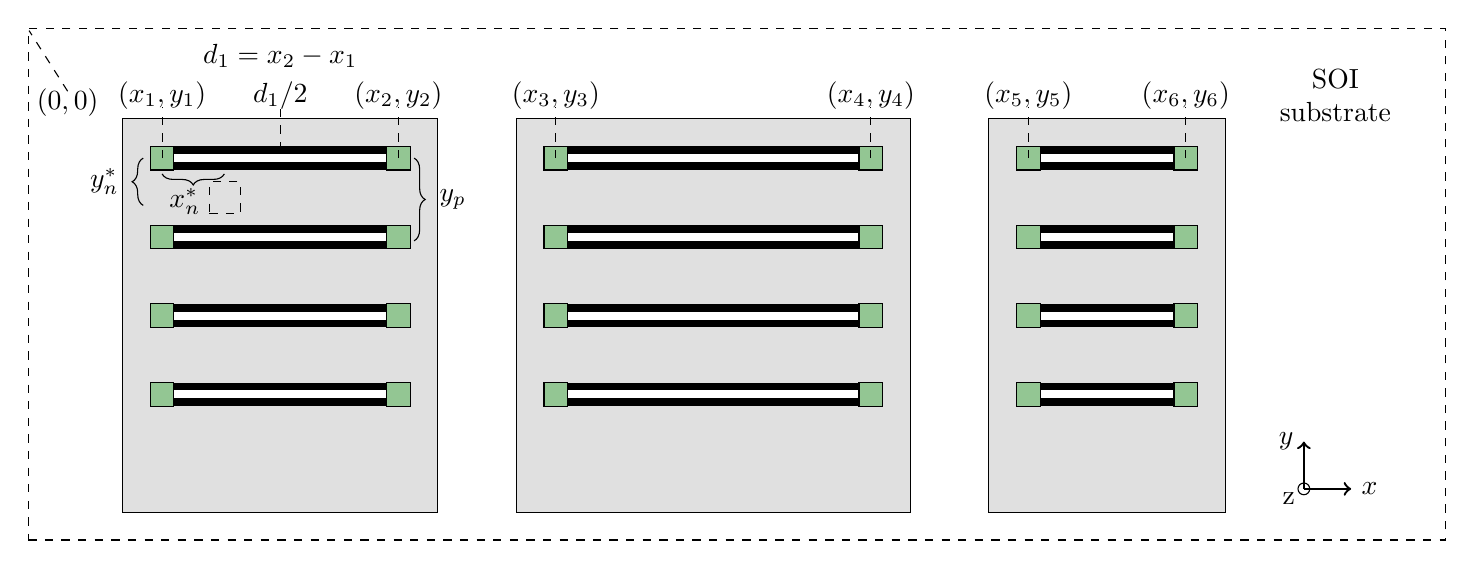
\begin{tikzpicture}
   	%define colors
    \definecolor{bbblue}{rgb}{0.262,0.709,0.613}
    \definecolor{rrred}{rgb}{0.933, 0.227, 0.286}
    \definecolor{yyyellow}{rgb}{0.933, 0.756, 0.227}
    \definecolor{gre}{rgb}{0.878, 0.878, 0.878}
    \definecolor{gre2}{rgb}{0.578, 0.778, 0.578}
    \definecolor{left} {HTML}{001528}
    %define coordinates for modulator (upper side)
    \coordinate (x1) at (-70.0mm, 20mm);
    \coordinate (x2) at (-40.0mm, 20mm);
    \coordinate (x3) at (-20.0mm, 20mm);
    \coordinate (x4) at (20.0mm, 20mm);
    \coordinate (x5) at (40.0mm, 20mm);
    \coordinate (x6) at (60.0mm, 20mm);
    
    \coordinate (D1) at (-55.0mm, 0);
    \coordinate (D3) at (50.0mm, 0); 
    \coordinate (ax) at (75mm, -22mm);
     
    % Substrate, modulators, Waveguides, MMI and converters %
    
    \node [shape=rectangle, minimum width=180mm, minimum height=65mm, dashed, draw]
    (substrate) at (3mm,4mm) {};
    
    \node [shape=rectangle, minimum width=40mm, minimum height=50mm, 
    fill=gre, draw] (dev1) at(D1) {};
    \node [shape=rectangle, minimum width=50mm, minimum height=50mm, 
    fill=gre, draw] (dev2) at(0,0) {};
    \node [shape=rectangle, minimum width=30mm, minimum height=50mm, 
    fill=gre, draw] (dev3) at(D3) {};
    
    \draw  [line width=3.00mm, color=black] (x1) -- (x2);
    \draw  [line width=1.00mm, color=white] (x1) -- (x2);
    \draw  [line width=3.00mm, color=black] (x3) -- (x4);
    \draw  [line width=1.00mm, color=white] (x3) -- (x4);
    \draw  [line width=3.00mm, color=black] (x5) -- (x6);
    \draw  [line width=1.00mm, color=white] (x5) -- (x6);
    
    \draw  [line width=3.00mm, color=black] ($(x1)-(0,10mm)$) -- ($(x2)-(0,10mm)$);
    \draw  [line width=1.00mm, color=white] ($(x1)-(0,10mm)$) -- ($(x2)-(0,10mm)$);
    \draw  [line width=3.00mm, color=black] ($(x1)-(0,20mm)$) -- ($(x2)-(0,20mm)$);
    \draw  [line width=1.00mm, color=white] ($(x1)-(0,20mm)$) -- ($(x2)-(0,20mm)$);
    \draw  [line width=3.00mm, color=black] ($(x1)-(0,30mm)$) -- ($(x2)-(0,30mm)$);
    \draw  [line width=1.00mm, color=white] ($(x1)-(0,30mm)$) -- ($(x2)-(0,30mm)$);
    
    \draw  [line width=3.00mm, color=black] ($(x3)-(0,10mm)$) -- ($(x4)-(0,10mm)$);
    \draw  [line width=1.00mm, color=white] ($(x3)-(0,10mm)$) -- ($(x4)-(0,10mm)$);
    \draw  [line width=3.00mm, color=black] ($(x3)-(0,20mm)$) -- ($(x4)-(0,20mm)$);
    \draw  [line width=1.00mm, color=white] ($(x3)-(0,20mm)$) -- ($(x4)-(0,20mm)$);
    \draw  [line width=3.00mm, color=black] ($(x3)-(0,30mm)$) -- ($(x4)-(0,30mm)$);
    \draw  [line width=1.00mm, color=white] ($(x3)-(0,30mm)$) -- ($(x4)-(0,30mm)$);

    \draw  [line width=3.00mm, color=black] ($(x5)-(0,10mm)$) -- ($(x6)-(0,10mm)$);
    \draw  [line width=1.00mm, color=white] ($(x5)-(0,10mm)$) -- ($(x6)-(0,10mm)$);
    \draw  [line width=3.00mm, color=black] ($(x5)-(0,20mm)$) -- ($(x6)-(0,20mm)$);
    \draw  [line width=1.00mm, color=white] ($(x5)-(0,20mm)$) -- ($(x6)-(0,20mm)$);
    \draw  [line width=3.00mm, color=black] ($(x5)-(0,30mm)$) -- ($(x6)-(0,30mm)$);
    \draw  [line width=1.00mm, color=white] ($(x5)-(0,30mm)$) -- ($(x6)-(0,30mm)$);
    % Meniscus formation offset
    \node [shape=rectangle, minimum width=4mm, minimum height=4mm, dashed, draw]
    (substrate) at ($(x1)-(-8mm,5mm)$) {};
        
   \node [shape=rectangle, minimum width=3mm, minimum height=3mm, draw,fill=gre2]
   (substrate) at (x1) {};
   \node [shape=rectangle, minimum width=3mm, minimum height=3mm, draw,fill=gre2]
   (substrate) at ($(x1)-(0,10mm)$) {};

    \node [shape=rectangle, minimum width=3mm, minimum height=3mm, draw,fill=gre2]
   (substrate) at ($(x1)-(0,20mm)$) {};
    \node [shape=rectangle, minimum width=3mm, minimum height=3mm, draw,fill=gre2]
   (substrate) at ($(x1)-(0,30mm)$) {};
   \node [shape=rectangle, minimum width=3mm, minimum height=3mm, draw,fill=gre2]
   (substrate) at (x2) {};
   \node [shape=rectangle, minimum width=3mm, minimum height=3mm, draw,fill=gre2]
   (substrate) at ($(x2)-(0,10mm)$) {};
   \node [shape=rectangle, minimum width=3mm, minimum height=3mm, draw,fill=gre2]
   (substrate) at ($(x2)-(0,20mm)$) {};
   \node [shape=rectangle, minimum width=3mm, minimum height=3mm, draw,fill=gre2]
  (substrate) at ($(x2)-(0,30mm)$) {};

   \node [shape=rectangle, minimum width=3mm, minimum height=3mm, draw,fill=gre2]
   (substrate) at (x3) {};
   \node [shape=rectangle, minimum width=3mm, minimum height=3mm, draw,fill=gre2]
   (substrate) at ($(x3)-(0,10mm)$) {};
    \node [shape=rectangle, minimum width=3mm, minimum height=3mm, draw,fill=gre2]
   (substrate) at ($(x3)-(0,20mm)$) {};
    \node [shape=rectangle, minimum width=3mm, minimum height=3mm, draw,fill=gre2]
   (substrate) at ($(x3)-(0,30mm)$) {};
   \node [shape=rectangle, minimum width=3mm, minimum height=3mm, draw,fill=gre2]
   (substrate) at (x4) {};
   \node [shape=rectangle, minimum width=3mm, minimum height=3mm, draw,fill=gre2]
   (substrate) at ($(x4)-(0,10mm)$) {};
   \node [shape=rectangle, minimum width=3mm, minimum height=3mm, draw,fill=gre2]
   (substrate) at ($(x4)-(0,20mm)$) {};
   \node [shape=rectangle, minimum width=3mm, minimum height=3mm, draw,fill=gre2]
  (substrate) at ($(x4)-(0,30mm)$) {};

   \node [shape=rectangle, minimum width=3mm, minimum height=3mm, draw,fill=gre2]
   (substrate) at (x5) {};
   \node [shape=rectangle, minimum width=3mm, minimum height=3mm, draw,fill=gre2]
   (substrate) at ($(x5)-(0,10mm)$) {};
    \node [shape=rectangle, minimum width=3mm, minimum height=3mm, draw,fill=gre2]
   (substrate) at ($(x5)-(0,20mm)$) {};
    \node [shape=rectangle, minimum width=3mm, minimum height=3mm, draw,fill=gre2]
   (substrate) at ($(x5)-(0,30mm)$) {};
   \node [shape=rectangle, minimum width=3mm, minimum height=3mm, draw,fill=gre2]
   (substrate) at (x6) {};
   \node [shape=rectangle, minimum width=3mm, minimum height=3mm, draw,fill=gre2]
   (substrate) at ($(x6)-(0,10mm)$) {};
   \node [shape=rectangle, minimum width=3mm, minimum height=3mm, draw,fill=gre2]
   (substrate) at ($(x6)-(0,20mm)$) {};
   \node [shape=rectangle, minimum width=3mm, minimum height=3mm, draw,fill=gre2]
  (substrate) at ($(x6)-(0,30mm)$) {};
       
    % Optical path %

    \node [align=center] (x1y1) at ($(x1)+(0,8mm)$) {$(x_1,y_1)$};
    \node [align=center] (x2y2) at ($(x2)+(0,8mm)$) {$(x_2,y_2)$};
    \node [align=center] (x3y3) at ($(x3)+(0,8mm)$) {$(x_3,y_3)$};
    \node [align=center] (x4y4) at ($(x4)+(0,8mm)$) {$(x_4,y_4)$};
    \node [align=center] (x5y5) at ($(x5)+(0,8mm)$) {$(x_5,y_5)$};
    \node [align=center] (x6y6) at ($(x6)+(0,8mm)$) {$(x_6,y_6)$}; 
    \draw [decorate,decoration={brace,amplitude=4pt},xshift=-6pt,yshift=0pt]  ($(x2)+(2mm,0mm)$) -- ($(x2)+(2mm,-10.5mm)$) node [black,midway,xshift=14pt] {$y_p$};
   \draw [decorate,decoration={brace,amplitude=4pt},xshift=-6pt,yshift=0pt]  ($(x1)+(-2.4mm,-6mm)$) -- ($(x1)+(-2.4mm,0mm)$) node [black,midway,xshift=-14pt] {$y^*_n$};
   \draw [decorate,decoration={brace,amplitude=4pt},xshift=-6pt,yshift=0pt] ($(x1)+(7.9mm,-2mm)$) -- ($(x1)+(0mm,-2mm)$) node [black,midway,xshift=-3pt,yshift=-10pt] {$x^*_n$};

    \node [align=center] (xp5) at ($(x1)+(15mm,8mm)$) {$d_1/2$};
    \node [align=center] (x1y1) at ($(x1)+(15mm,13mm)$) {$d_1 = x_2 - x_1$};	
    \node [align=center] (zpz) at ($(x1)+(-12mm,7mm)$) {$(0,0)$};
	
	\draw [dashed] ($(x1)  - (12mm, -8.5mm)$) -- ($(x1)  + (-16.9mm, +16.2mm)$);
    \draw [dashed] ($(x1)  - (0mm, 0mm)$) -- ($(x1)  + (0mm, 6.5mm)$);
    \draw [dashed] ($(xp5)  - (0mm, 7mm)$) -- ($(xp5)  + (0mm, -1mm)$);
    \draw [dashed] ($(x2)  - (0mm, 0mm)$) -- ($(x2)  + (0mm, 6.5mm)$);
    \draw [dashed] ($(x3)  - (0mm, 0mm)$) -- ($(x3)  + (0mm, 6.5mm)$);
    \draw [dashed] ($(x4)  - (0mm, 0mm)$) -- ($(x4)  + (0mm, 6.5mm)$);
    \draw [dashed] ($(x5)  - (0mm, 0mm)$) -- ($(x5)  + (0mm, 6.5mm)$);
    \draw [dashed] ($(x6)  - (0mm, 0mm)$) -- ($(x6)  + (0mm, 6.5mm)$);
	
	\node [align=center] (soi) at ($(x6)+(19mm,8mm)$) {SOI\\substrate};

%axes
 \node [shape=circle, color=black, fill=white, inner sep=1.5, draw]
    (substrate) at (ax) {};
 \draw (ax) node [text width=3mm] (axx) at + (-1.2mm,-1.2mm) {z};
 \draw [->, to path={-| (\tikztotarget)},line width=0.30mm, color=black, draw]  (ax) -- ($(ax) + (0,6mm)$) node[left] {$y$};
 \draw [->, to path={-| (\tikztotarget)},line width=0.30mm, color=black, draw]  (ax) -- ($(ax) + (6mm,0)$) node[right] {$x$};
  \end{tikzpicture}
%  \caption{Schematische Darstellung eines in Lithiumniobat (LiNbO$_3$) realisiertes
%  Mach-Zehnder-Modulators.}
%  \label{fig:mzm}
%\end{figure}
\end{document}